\documentclass[a4paper,11pt]{book}
\usepackage{import}
\usepackage{preamb}

\makeindex

\begin{document}

\small
\begin{multicols}{3}

%\maketitle

\thispagestyle{empty}
\scriptsize
\newpage


\begin{subbox}{subbox}{}
\centering
\Large{\textbf{Network Science   \\ Cheatsheet}}
\end{subbox}

\begin{multibox}{2}
\begin{subbox}{subbox}{}
\centering

\includegraphics[width=0.8\textwidth]{pics/logo.png}
\end{subbox}
\begin{subbox}{subbox}{}
\centering
Made by \\
\large{
Remy Cazabet
}
\end{subbox}
\end{multibox}
% \section{Blocks and Community structure}


\begin{subbox}{subbox}{}
\centering
\Large{\textbf{Spatial Networks}}
\end{subbox}




\begin{textbox}{Definition}
A spatial network is a network in which 1)Nodes are associated to positions, 2) The probability of observing edges between a pair of nodes depends on their distance.

In most cases, the probability of being connected tends to decrease with distance, but this is not a necessary requirement.

\end{textbox}


\begin{textbox}{Position of nodes - Dimension}
The position of each node is described by a vector, i.e., a list of values. The number of values in the vector is the \textbf{dimension}(d) of the space in which nodes are located. The most common space is \textit{geographical space}: nodes are located by a pair \textbf{(latitude, longitude)}. It is therefore considered a 2D space (even though earth is spherical). But spatial networks can exist in spaces with more or less dimensions, as long as the distance between nodes positions is meaningful.
\end{textbox}


\begin{textbox}{Examples of 1D spaces}
\begin{itemize}
    \item The Watts-Strogatz random graph is defined on a (circular) 1D space: each node is (initially) connected to its $k$ closest nodes in this space. 
    \item In social networks, users tend to be more connected with other users with similar age. We can consider $age$ as a position on a 1D space. The same is true about political opinions, if we consider a Left-Right spectrum.
\end{itemize}
\end{textbox}




\begin{textbox}{Examples of 3+D spaces}
\begin{itemize}
    \item If we consider altitude, geographical networks are 3D spaces. Neurons in the brain, atoms in proteins are also embedded in 3D spaces.
    \item If we consider multiple nodes properties as dimensions, nodes can be located on high dimensional spaces, e.g., age, political opinion, revenue, geographical location, etc. Be careful however, that analyzing a spatial networks needs to define the \textit{distance} between nodes, which can be tricky to define if dimensions are of different natures.
    \item Methods such as \textit{graph embedding} assign to nodes locations in an arbitrary number (e.g., 128) of dimensions that summarize some of the network properties (see later class).
\end{itemize}


\end{textbox}

\begin{textbox}{Distances}
The distance between each pair of nodes can be computed in different ways, depending on the nature of dimensions nodes are embedded in. The most common ones are:
\begin{itemize}
    \item \textbf{Euclidean distance}, or $L^2 distance$ is the usual, straight line distance
    \item \textbf{Great-Circle distance} is used to measure the distance between points located on a sphere, typically the Earth for geographical data.
    \item \textbf{Dot product} and \textbf{Cosine Distance} are often used in high dimensions, in particular when it makes sense to multiply the location vectors.
    \item \textbf{Manhattan distance}, or $L^1 distance$, is sometimes used as a variant of Euclidean distance for high dimensional data (it is simply defined as the sum of differences in each of the dimensions.)
    \item Observed distances can sometimes be used, a typical example being \textbf{average time distance}: in datasets of trips or traffic, the time distance between dots might be only loosely proportional to geographical distance.
\end{itemize}


\end{textbox}






\begin{textbox}{Metric Space}
In most cases, we can consider that a spatial network is embedded in a \textbf{metric space}, a space associated with a metric with properties of \textit{indiscernibility}, \textit{symmetry} and \textit{triangle inequality}. However, this is not always the case, in particular in directed networks, in which it can be useful to consider different distances for links $(a,b)$ and $(b,a)$ (asymmetry). 


\end{textbox}



\begin{textbox}{Notation}
\begin{tabular}{p{0.12\textwidth}|p{0.8\textwidth}}\scriptsize
$\Delta_{uv}$ & \textbf{Metric distance} between $u$ and $v$ (Euclidean, Manhattan, etc.)\\
$\ell_{uv}$ & \textbf{Route distance} between $u$ and $v$, i.e., sum of Metric distances between nodes on the shortest path between $u$ and $v$\\
$s_u^\Delta$ & \textbf{Distance strength}, cumulative distance from a node to its neighbors. $s_u^\Delta=\sum_{v \in N(u)}\Delta_{uv}$. The relation between $k_u$ and $s_u^\Delta$ can be studied, for instance to see if larger nodes tend to connect at longer distances.

\end{tabular}


\end{textbox}



\begin{textbox}{Route factor - Accessibility}

\begin{tabular}{p{0.09\textwidth}|p{0.8\textwidth}}\scriptsize
$Q(u,v)$ & \textbf{Route Factor}, also called the detour index, measures how \textit{efficiently} the network allows to go from a node to another, it is defined as the ratio between the metric distance and the route distance: \[Q(u,v)=\frac{\Delta_{uv}}{\ell_{uv}}\] \\
$\langle Q(u)\rangle$ & \textbf{Node Accessibility}: Average route factor from a node to all others: \[\langle Q(u)\rangle=\frac{1}{N-1}\sum_v Q(u,v)\]\\
$\langle Q\rangle$ & \textbf{Accessibility}: Average route factor for the whole network: \[\langle Q\rangle=\frac{1}{N(N-1)}\sum_{u\neq v} Q(u,v)\]\\
\end{tabular}

\end{textbox}





\begin{textbox}{Random Geometric Graphs (RGG)}
\textbf{Random Geometric graphs} (RGG), also called Disk-percolation random graphs, are defined as such:
\begin{itemize}
    \item Distribute $n$ nodes randomly on a bounded $d$ dimensional space.
    \item Connect any two nodes at distance less than a parameter $r$
\end{itemize}

Properties\footcite{dall2002random} are:

\textbf{Degree distribution}: Poissionan, as ER random graphs.

\textbf{Clustering coefficient} (in large graphs): $C=3\sqrt{\frac{2}{\pi d}}(\frac{3}{4})^{\frac{d+1}{2}}$. It does not depend on the number of nodes, unlike random graphs, thus is not vanishing with network size for fixed average degree.

\end{textbox}


\begin{textbox}{Soft RGG (Waxman random graph)}
\textbf{Soft RGG}, or \textbf{Waxman Random Graphs}\footcite{waxman1988routing}, starts as the RGG by distributing nodes at random in a space, but instead of adding links between all nodes closer than a certain distance, it assign edges between nodes according to a \textbf{deterrence function} $f$, i.e., a function defining how distance affects the probability of observing edges between nodes.

The Soft RGG can model an ER random graph if  $f$ is a constant function, $f(\Delta)=p$.
It can model a classic RGG if $f$ is a threshold function with:
\[
f(d)=\begin{cases} 
      1 & \Delta\leq r \\
      0 & \Delta> r \\
   \end{cases}
\]
\end{textbox}









\begin{textbox}{Deterrence function}
A deterrence function defines how the distance affects the probability of observing an edge.
It can describe probabilities of connections at a given distance, or define a ratio of change compared with a null model.

\begin{enumerate}
    \item It can be defined \textit{a priori}, usually as a classic monotonically decreasing function, e.g., Negative exponential($f(\Delta)=e^{-\alpha\Delta}$) or Negative power ($f(\Delta)=\Delta^{-\alpha}$), with $\alpha$ a parameter. A typical example of negative power in geographical data is when the probability of observing an edge decreases as the square of the distance, i.e., $f(\Delta)=\frac{1}{\Delta^2}$
    \item It can also be learned from data, either by fitting parameters of a predefined function (e.g., the $\alpha$ parameter above), or by using an \textit{Ad-Hoc deterrence function}.
\end{enumerate}

\end{textbox}




\begin{textbox}{Ad-Hoc deterrence function}
When a spatial model is used to create a randomized version of an observed network, the most appropriate deterrence function can be learned from data. A simple way to achieve this is to count the fraction of edges occurring between nodes at a given distance, and to compare it with edges that should appear at random if there was no spatial effect. To avoid overfitting (each pair of node being at different distances with infinite precision), we usually create \textit{bins} of relevant size, e.g., every cm, km, 100km, etc., or using bins of exponentially growing size, e.g., {[0,1],[1,3],[3,7],[7,15],[15,31]}.

More formally, the deterrence function for each distance $\delta$ is defined as:
% \[
% f(d)=\frac{|{(u,v)\in E,d_M(u,v)=d|}}{\sum_{u,v \in V, d_M(u,v)=d}p(u,v)}
% \]
\[
f(\delta)=\frac{\sum_{i,j|\Delta_{ij}=\delta}A_{ij}}{\sum_{i,j|\delta_{ij}=\delta}M_{ij}}
\]
with $A_{ij}$ the adjacency matrix (or weight matrix) of the observed graph and $M_{ij}$ the probability of observing an edge (or weight of edges) between nodes $i$ and $j$ according to the chosen null model. For instance, with the simplest hypothesis that edges occur completely at random, $\forall_{i,j},M_{ij}=d$ (with $d$ the network density).
\end{textbox}

\begin{textbox}{Non monotony of deterrence function}
In a variety of real situations, ad-hoc deterrence functions are non-monotonous. Think of car trips, plane trips, bicycle trips, etc. It is not efficient to use such transportation systems for trips shorter than a given distance, and thus the deterrence function is initially increasing, until reaching the distance of optimal efficiency, from which the function start decreasing.
\end{textbox}






% \begin{textbox}{Spatial Preferential Attachment}
% The \textbf{Spatial Preferential Attachment} random graph model combines Barabasi-Albert Random Graphs and the Soft RGG. Nodes are added one after the other at random positions in a bounded space, and they create edges with other nodes with a probability $p(\Delta,k)=k f(\Delta)$, with  $f(\Delta)$ a deterrence function. The model has notably been studied with $f(\Delta)=d^\alphga$, with $\alpha$ a parameter. In this case, it can be shown that the network is scale-free if $\alpha>-1$.

% \end{textbox}



\begin{textbox}{Gravity Model of Spatial Interactions}
The Gravity Model of Spatial Interaction has been known for a long time in Geography. It is defined by analogy with Newton's law of gravitation and, in its original form, says that the strength of the relation between two places (countries, cities, etc.) is proportional to they \textit{power of attraction} $P$ and to the inverse of their distance. More formally, the expected strength of interaction $G_{ij}$ between locations $i$ and $j$ is:
\[
G_{ij}=K\frac{P_i^{out}P_j^{in}}{\Delta_{ij}^2}
\]

Common examples would be a model of a job market between cities, with $P_i^{in}$ the number of jobs offered in city $i$ and $P_i^{out}$ the number of job seekers in city $i$. $K$ is a normalization constant.
\end{textbox}



\begin{textbox}{Relaxed Gravity Model}
The gravity model can be relaxed to accept any deterrence function, chosen $a priori$ or fitted on data. The important difference with a soft RGG is that the probability of observing interactions is \textbf{proportional to the attractiveness of entities}. More formally:
\[
G_{ij}=P_i^{out}P_j^{in}f(\Delta_{ij})
\]
\end{textbox}




\begin{textbox}{Network Gravity Model}
The gravity model naturally translates as a \textbf{Spatial Configuration Model}, by considering that the degree of nodes correspond to their power of attraction. It is intuitively expressed in network terms as follows: each of the out-going stub of node $i$ connects at random with an in-going stub of all other nodes, with a probability biased by the deterrence function.
\end{textbox}

\begin{textbox}{Deterrence function in Gravity Model}
The custom deterrence function of a graph that we want to model using a Gravity Model can be expressed as:

\[
f(\delta)=\frac{\sum_{i,j|\delta_{ij}=d}A_{ij}}{\sum_{i,j|\delta_{ij}=\delta}\frac{k_ik_j}{2L}}
\]

This is because the probability to observe edges between two nodes without spatial effect is defined by the Configuration Model.

\end{textbox}



\begin{textbox}{Degree-Preserving Gravity Model}
A weakness of the network gravity model is that it does not preserve degrees: if we consider two nodes for which we have observed a same degree $k$, one located in the center of space, and thus having many other nodes at positively biased distances, and the other at the periphery having fewer nodes at those distances, the peripheral node will having fewer edges according to the network model than the central one. A solution\footcite{cazabet2017enhancing} to correct this is to fit nodes \textit{attractiveness} that would best explain the observed degrees, for a given graph and a given deterrence function.
\end{textbox}






\begin{textbox}{Radiation Law of Spatial Interactions}
The \textbf{Radiation Law}\footcite{simini2012universal} is another random spatial model. Unlike previous ones, it does not depends on a deterrence function, and is parameter-free. It is based on the principle of relative opportunities: the probability of observing an interaction from $i$ to $j$ depends on $P_i^{out}$, $P_j^{in}$, and the sum of all $P_k^{in}$ for $\Delta_{ik}<\Delta_{ik}$, i.e., other opportunities accessible at a shorter distance.
More formally:

\[
R_{ij}=k_i^{out}\frac{P_i^{out} P_j^{in}}{(P_i^{out}+s_{ij})(P_i^{out}+P_j^{in}+s_{ij})}
\]

With $s_{ij}=\sum\limits_{u\in V,\Delta_{iu}<\Delta_{ij}}P_u^{in}$ the sum of opportunities at a shorter distance than the target. 
\end{textbox}






\begin{textbox}{Radiation Law of Spatial Interactions}
Illustration of the zone $s_{ij}$ in which opportunities decrease the probability of interactions between $i$ and $j$.
\centering
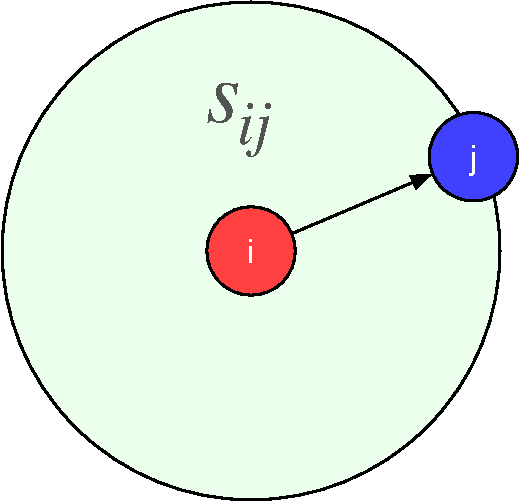
\includegraphics[width=0.4\textwidth]{pics/radiation.pdf}

\end{textbox}



\begin{textbox}{Radiation Law VS Gravity Law}
The advantage of the radiation law compared with the gravity law is that two nodes located at the same distance and of similar degrees can have different edge probabilities depending on their surroundings. Intuitively, the expected relation between two small scale cities at distance $\delta$ is different if both cities are far from any other large town, or if a Metropolis lies between them. 

On the contrary, the weakness of the Radiation Law comes from its simplicity: without deterrence function, it is impossible to take into account non-linear and non-monotonic influence of the distance.
\end{textbox}





\begin{textbox}{Space-Corrected Community Detection}
Community detection applied to spatial networks tends to yield communities corresponding to a spatial partition of space, even if there is actually no \textit{boundary} between those regions. A method as been proposed\footcite{expert2011uncovering} to remove the influence of space, and thus discover communities corresponding to non-spatial (social, etc.) effects, usually hidden behind the influence of spatial constraints. The principle is to use a Modularity-maximization algorithm, in which the null-model used by Modularity (usually, a Configuration Model) is replaced by a spatial model (usually, a Gravity Model)

\centering
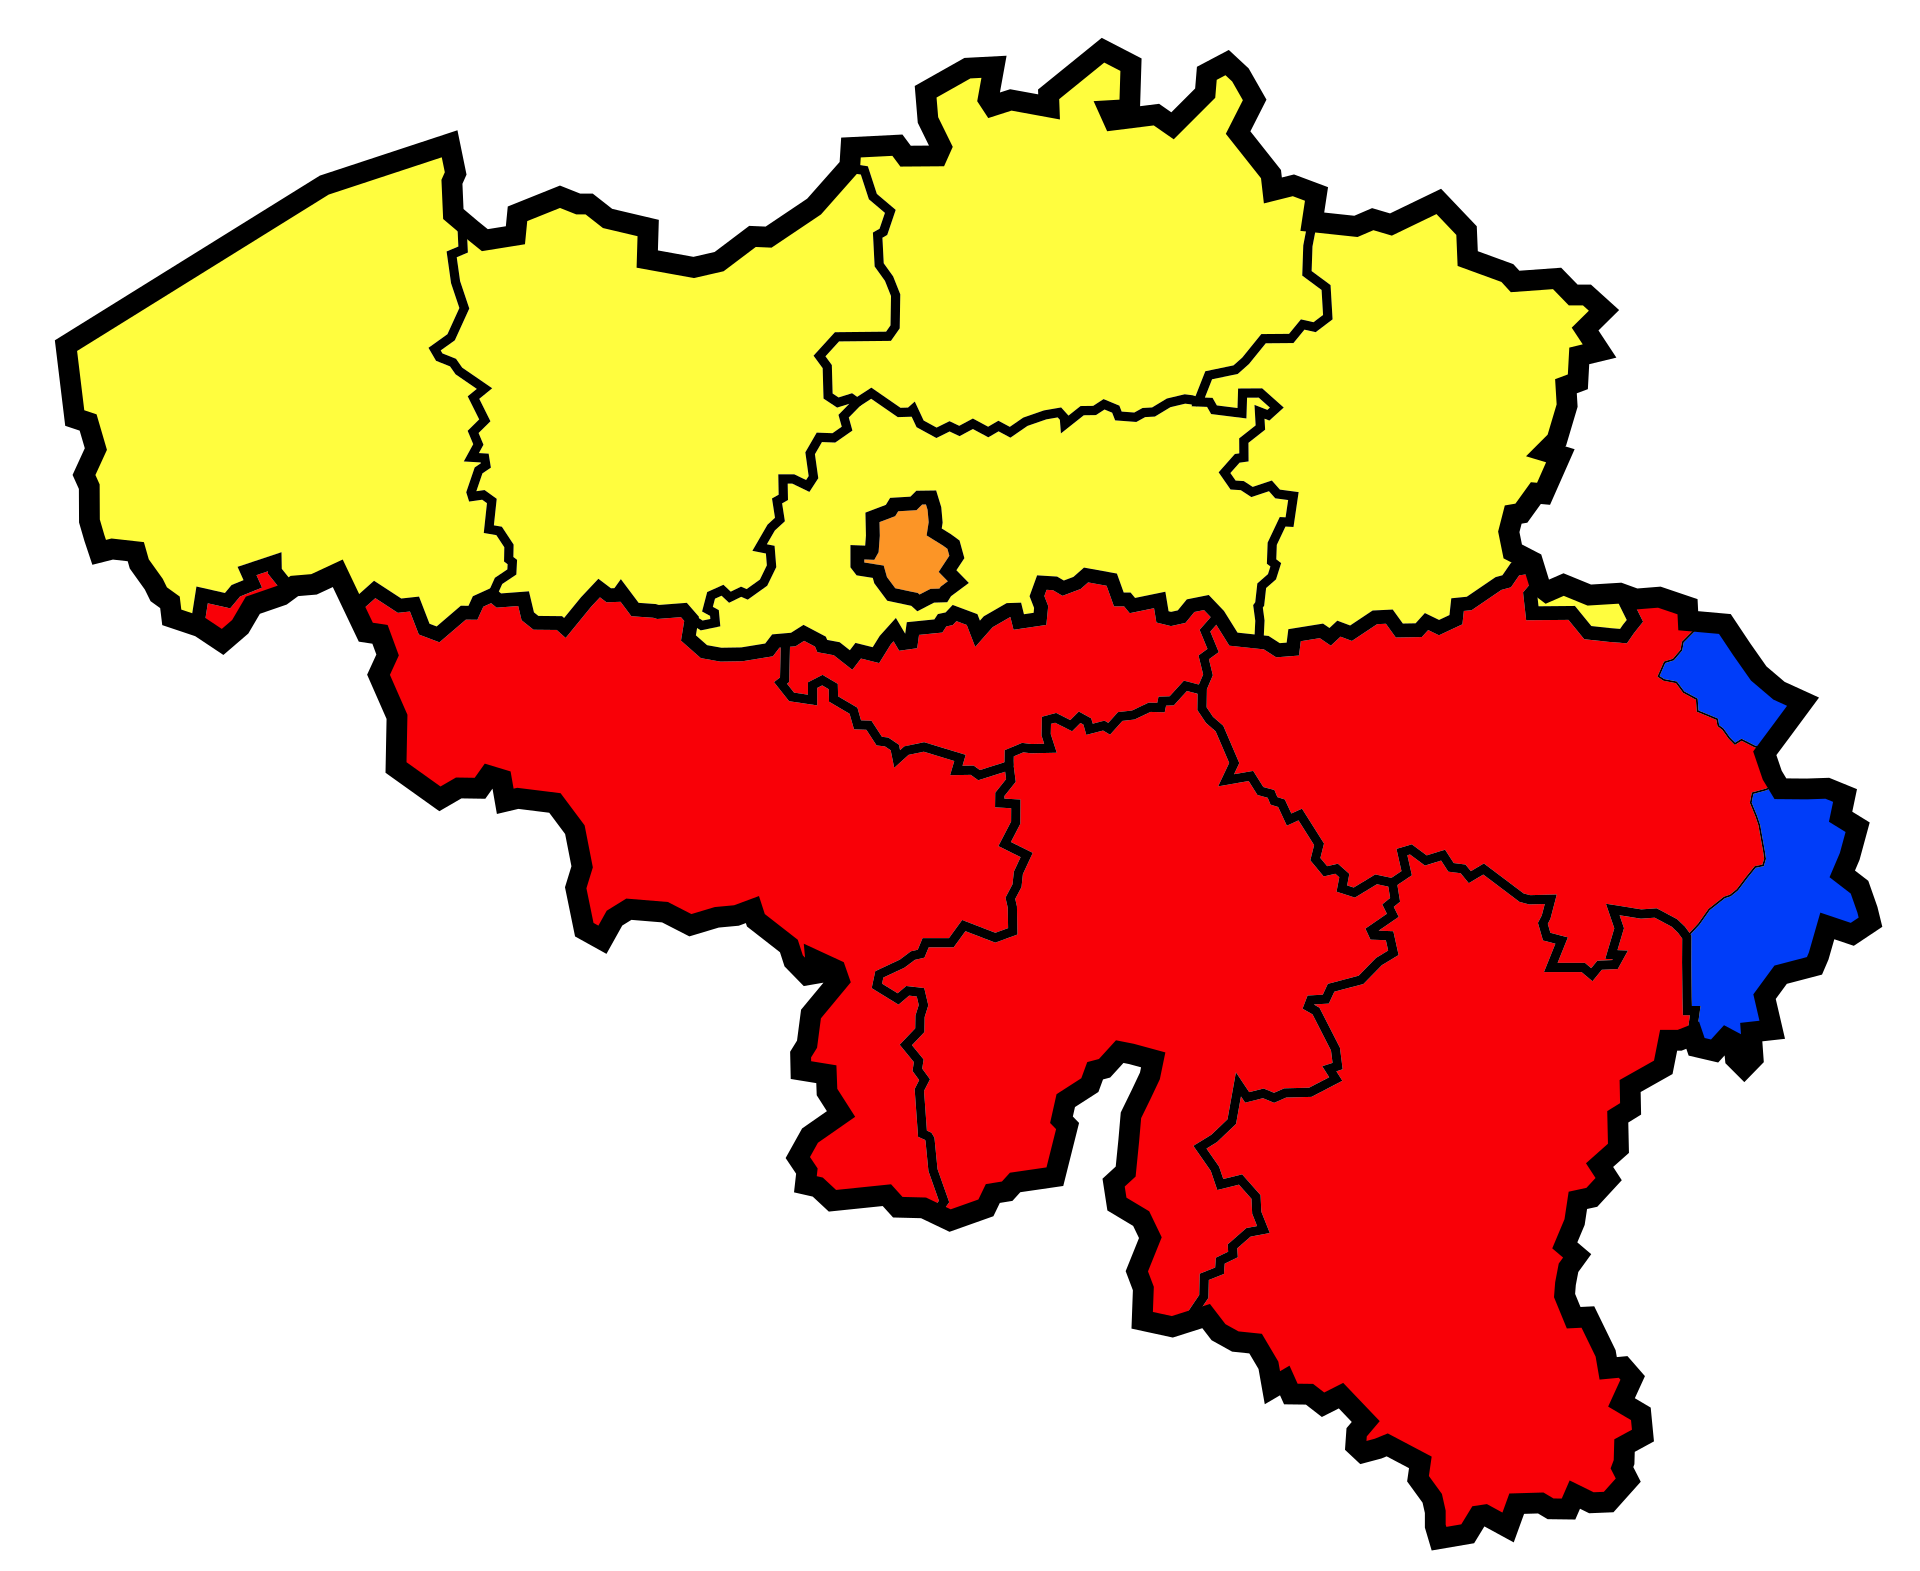
\includegraphics[width=0.4\textwidth]{pics/belgium.png}

Illustration: map of Belgium \footnote{\url{https://en.wikipedia.org/wiki/Communities,_regions_and_language_areas_of_Belgium}}. Black Lines could be find by community detection without spatial correction(geographic partitions). Colors could correspond to Space-corrected partition (linguistic partition).
\end{textbox}






\begin{textbox}{Going further}
Spatial Networks: (\cite{barthelemy2011spatial})
\end{textbox}

 \AtNextBibliography{\footnotesize}


\printbibliography[heading=subbibliography]


\end{multicols}



\end{document}


